
\chapter{ORGANIZATION}
      \section{History}
      Before joining bachelor's program by CEO, he was self-motivated, reading business model books and always focused on starting a company. In the 3rd year of his bachelor's degree, started their own company with a vision to contribute to society by teaching trending topics in technologies rather than being a client-service organization. Driven by a passion for entrepreneurship, the whole team actively hosted various tech occasions. Currently, they are excited about bioinformatics research.
      
      \section{Objectives}
      The company has the following objectives:
      \begin{itemize}
        \item Initial goal: Empowerment of the youths in entrepreneurship
        \item Convert to a corporate company
        \item Create events so that youth can showcase their talents
        \item Research in bioinformatics
      \end{itemize}

      \section{Working of Organization}
      \subsection{Input}
        \begin{itemize}
          \item Urja Lab has made a clear short-term and long-term strategy to meet their goals.
          \item The company has a very few to none competitor in the valley. They have performed market analysis to follow current trends, analyse competitors and anticipate customer needs.
          \item Company has a detailed financial policy, performs regular financial reporting. 
          \item Following the demands and industrial trends, human resources are recruited and proper training and development programs are set for them along with compensation and benefits.
          \item The company has Legal Advisor who provides legal advice when needed.
          \item Urja Lab does minimal marketing as it has already made its presence in the valley.
          \item Company provides a friendly environment and proper environment for everyone to communicate.
      \end{itemize}
      \subsection{Output}
      The company provides the following services:
      \begin{itemize}
        \item Brand Guidaeline and Development
        \item Digital Marketing
        \item Event Management
        \item Technical Support for Business
        \item Cources on UTA(Urja Tech Academy)
        \item Incubation and Enterpreneurship
        \item Human Resource Management
      \end{itemize}

      \section{Organizational Structure}
      Urja Lab has a functional organizational structure, which entails several layers of management that are in favor of a linear authority system. This arrangement promotes effective monitoring, making decisions, and assuring people. The detailed breakdown of the structure is shown below.
        \begin{enumerate}
           \item  \textbf{Top-Level Management}
            \begin{description}
                \item[\textbf{CEO:} ]  The CEO holds the highest authority within the company and is responsible for overall strategic planning, decision-making, and company oversight.
                
                
                \item[Legal Advisor: ]  The Legal Advisor handles all legal issues to make sure that the laws and rules are followed. They offer legal advice to the CEO as well as other departments, manage legal risks and administrate cases related to the company. 


                \item[Head Manager: ]  The Head Manager on the other hand is responsible for day to day operations in the company

                \item[CA(Chartered Accountant): ] The CA manages the financial operations of the company, including accounting, auditing, financial reporting, and budgeting. They ensure the financial health of the company and provide financial insights to support decision-making.
                 
            \end{description}
            
            \item \textbf{Middle Level Management}
            \begin{itemize}
            \begin{description}
                \item[Manager: ] The Manager ensure that their team meets performance targets and sticks to company policies. 
                \item[System Admin: ] The System Admin manages the IT infrastructure, including system maintenance, network security, and technical support ensuring that the company’s technology resources are efficient and secure from attackers.
                \item[HR (Human Resources) Manager:] The HR department handles recruitment, training, employee relations, ensuring company finds the best talent.
            \end{description}
            \end{itemize}
            \item \textbf{Operational Level}
            \begin{itemize}
            \begin{description}
                \item[Team Leader: ] The Team Leader supervise and guide their members to ensure the tasks and projects are completed efficiently and effectively meeting the requirements 
            \end{description}
            \end{itemize}
            \item \textbf{Execution Level}
            \begin{itemize}

            \begin{description}
                \item[Team Members:] Team Members are basically responsible for the execution of the company's dat to dat operations, carry out specific tasks and projects as provided by the team leader.
            \end{description}
            \end{itemize}
        \end{enumerate}
        \begin{figure}[H]
          
          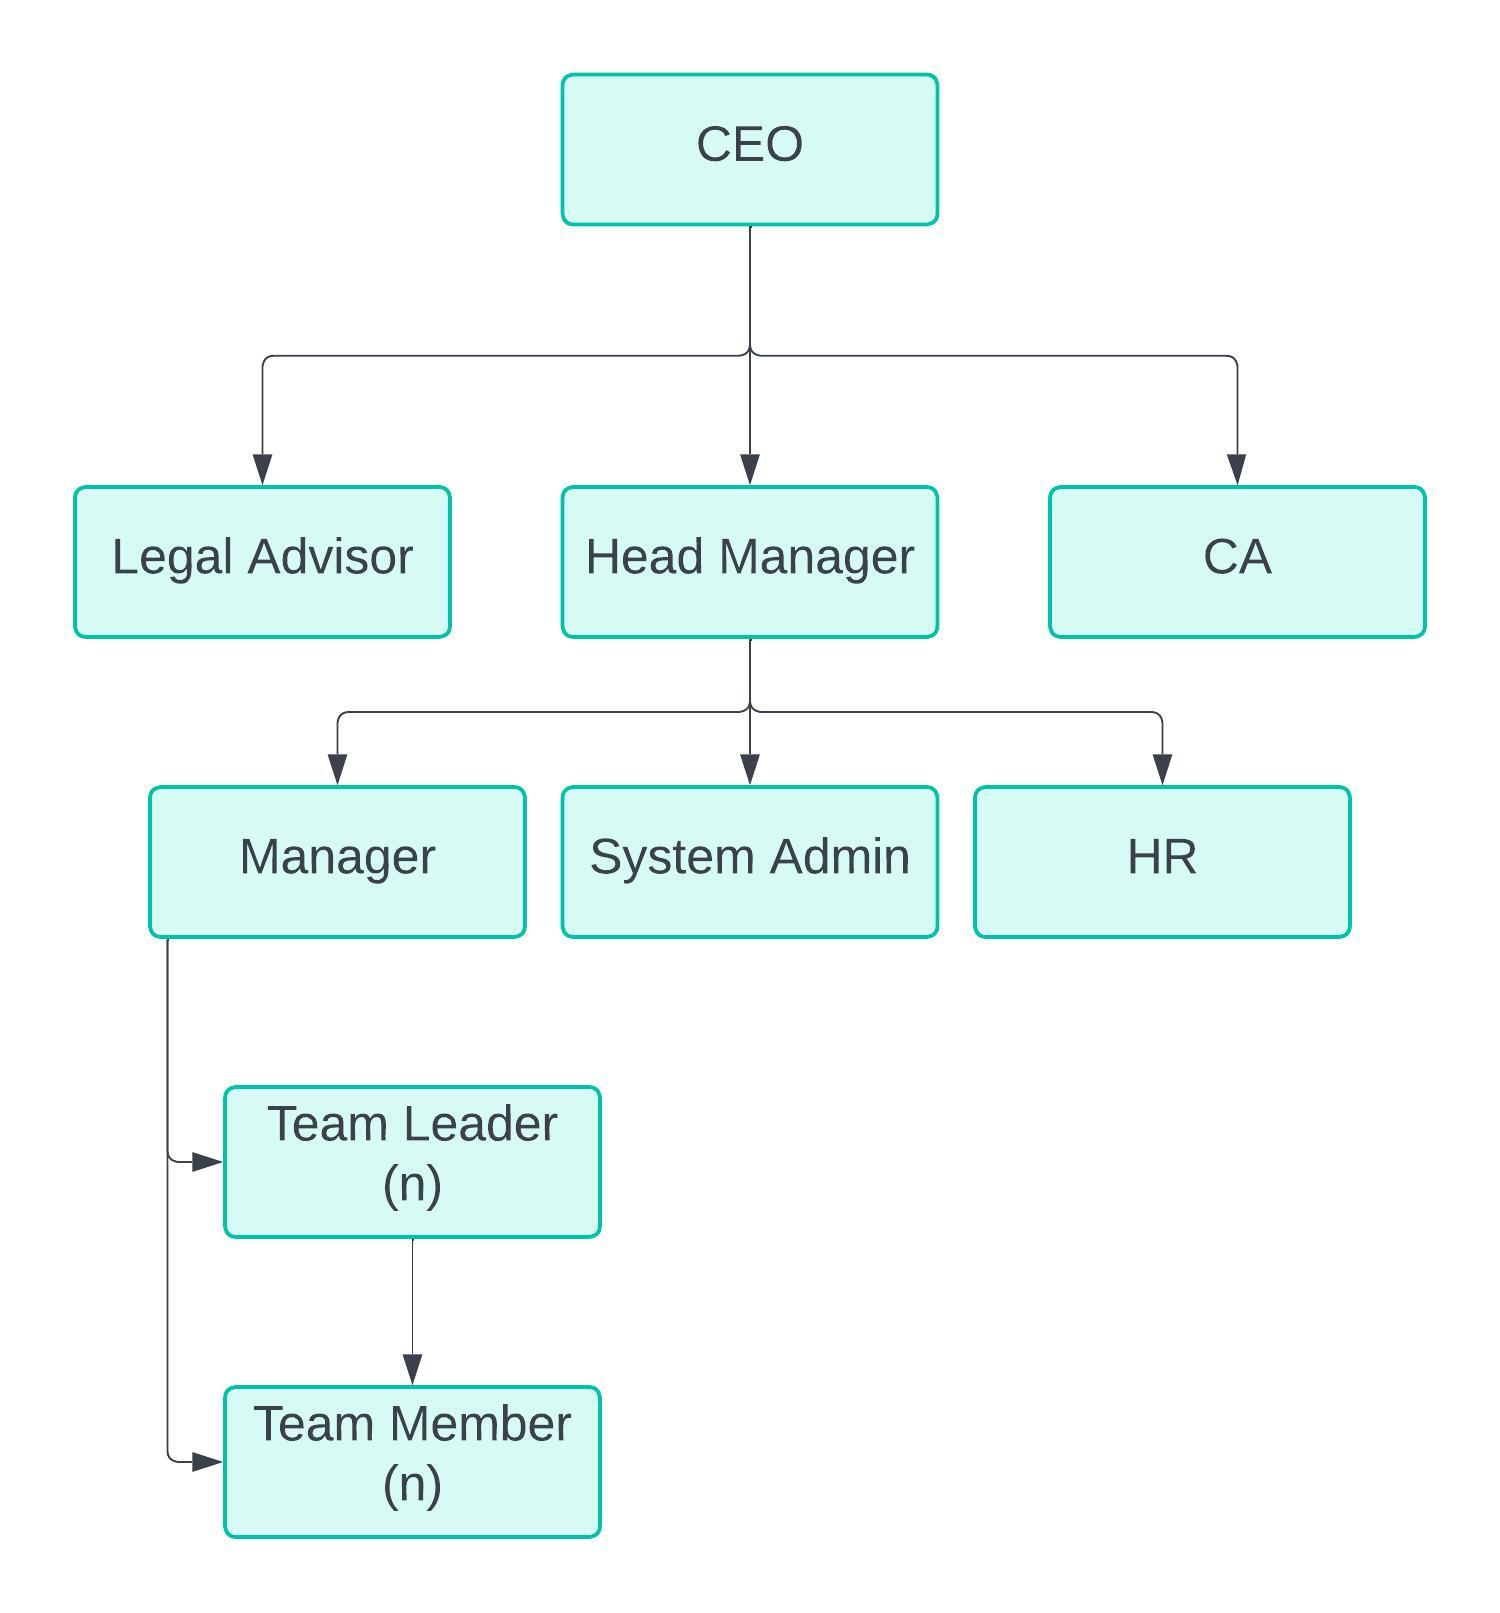
\includegraphics[width=\textwidth]{./Graphics/orgchart.jpeg}
          \caption{Organizational Structure of Urja Lab}
          \label{fig:orgchart}
        \end{figure}
        

      \section{Forms of Ownership}
This business operates similarly to a sole trader, where the company's head, often the Chief Executive Officer, is also the owner. This structure means there is little distinction between the owner's personal life and business decisions, making the owner accountable for the company's losses or obligations.

Despite being a sole trader, the business can still engage with other firms, including sibling companies. Sister companies are separate legal entities under the same ownership, commonly through a corporate group. These affiliations can involve various partnerships, such as mergers, strategic alliances, joint ventures, consignment, or franchising. These arrangements allow each entity to maintain its distinct legal and operational identity while cooperating for mutual benefit.

A sole proprietorship can partner with sister companies to share resources, cut costs, expand markets, or develop new products. Each business retains its individual identity but collaborates as part of a larger group. The partnerships vary depending on the relationships between the companies and their specific strategic goals, allowing for diverse forms of cooperation.
